\section{Příklad 1}
% Jako parametr zadejte skupinu (A-H)
\prvniZadani{G}

 
%%% Krok 1 
\begin{center}
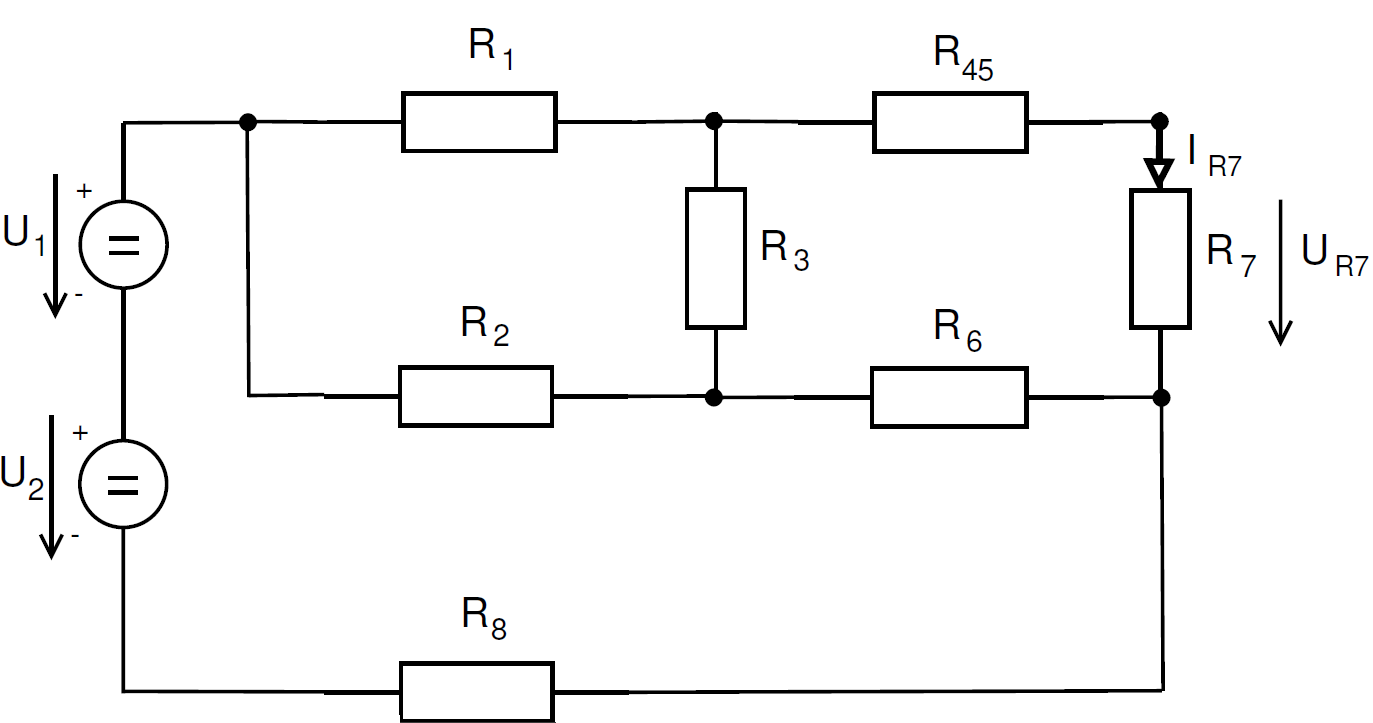
\includegraphics[scale=0.5,keepaspectratio]{fig/obr/Pr1_1.png} \\
\textbf{Krok 1} - Zjednodušenie $R_{4}$ a $R_{5}$ podľa vzorca pre paralelne zapojené rezistory.
\end{center}

\begin{gather*}
R_{45}=\frac{R_{4} \times R_{5}}{R_{4}+R_{5}}=\frac{440 \times 450}{440+450}=222,4719\Omega 
\end{gather*}



%%% Krok 2
\begin{center}
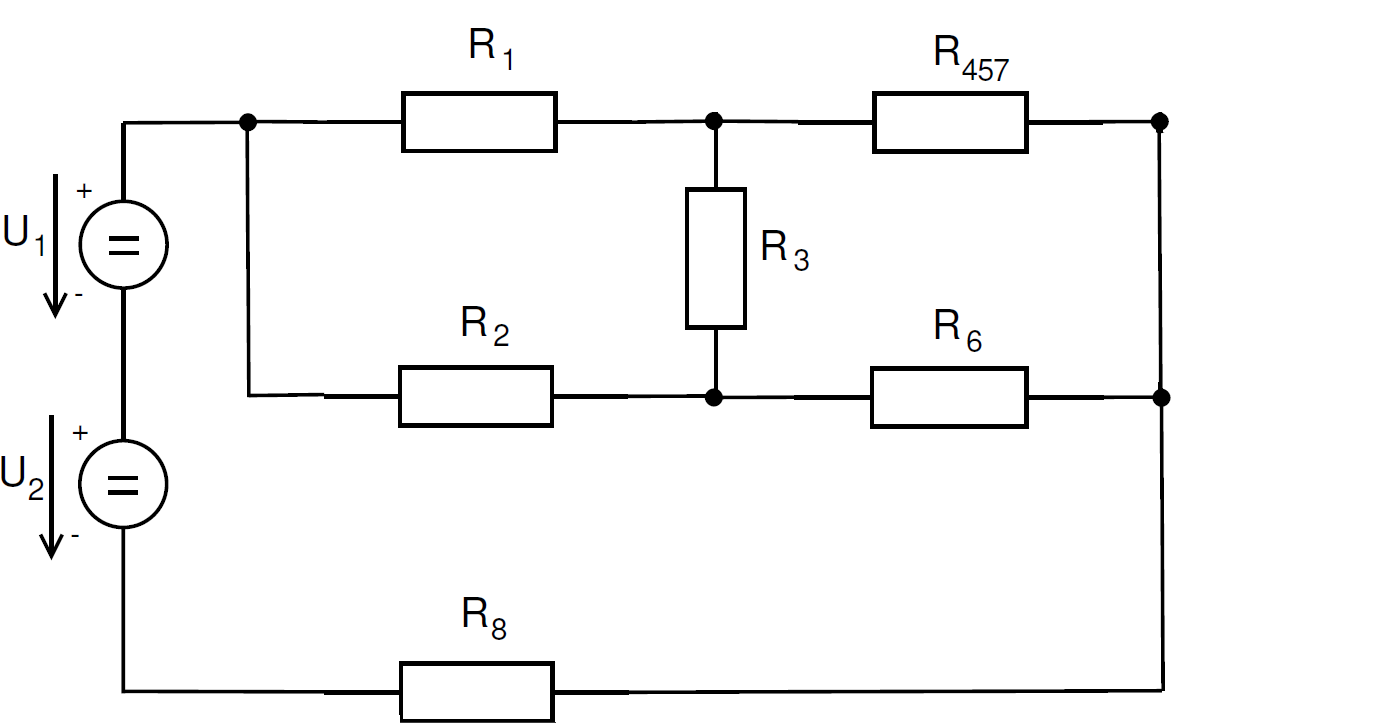
\includegraphics[scale=0.5,keepaspectratio]{fig/obr/Pr1_2.png} \\
\textbf{Krok 2} - Zjednodušenie $R_{45}$ a $R_{7}$ podľa vzorca pre sériovo zapojené rezistory.
\end{center}

\begin{gather*}
R_{457}=R_{45}+R_{7}=222,4719+410=632,4719\Omega 
\end{gather*}


%%% Krok 3
\begin{center}
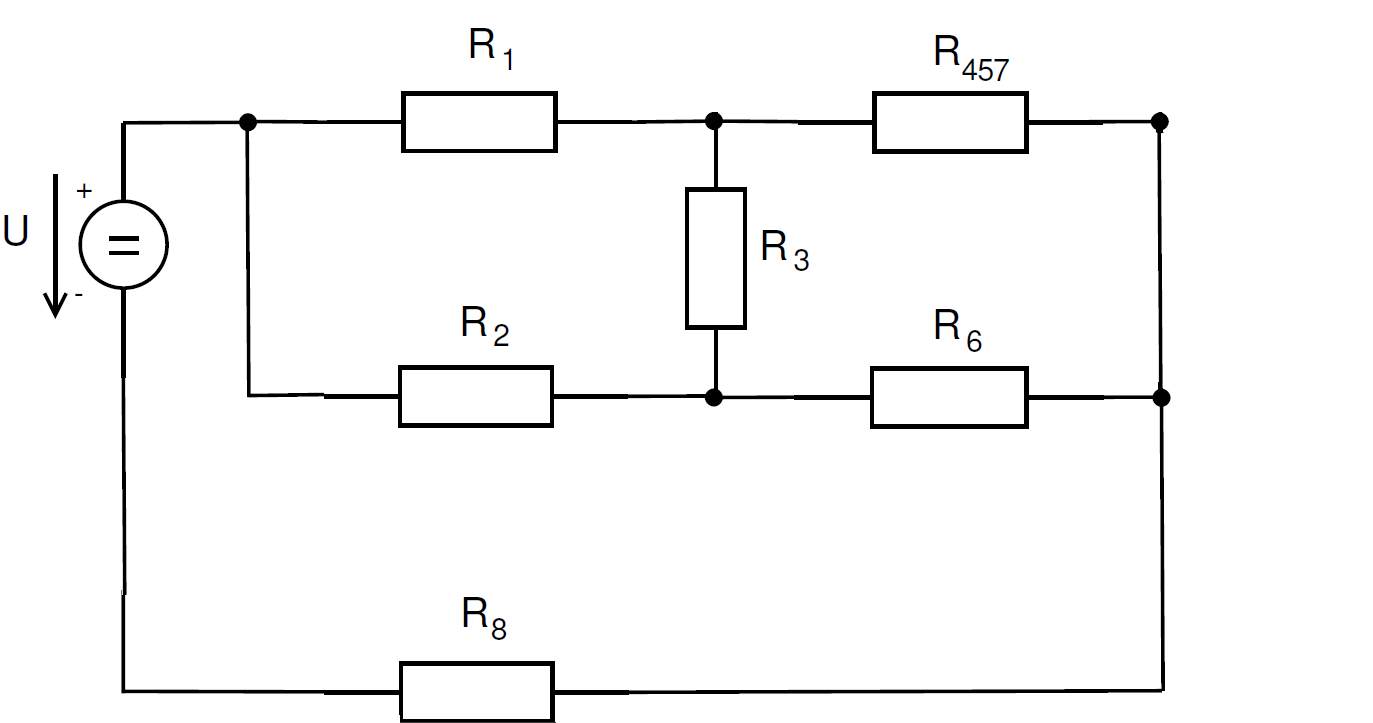
\includegraphics[scale=0.5,keepaspectratio]{fig/obr/Pr1_3.png} \\
\textbf{Krok 3} - Zjednodušenie napätia $U_{1}$ a $U_{2}$.
\end{center}

\begin{gather*}
U=U_{1}+U_{2}=130+60=190V 
\end{gather*}


%%% Krok 4
\begin{center}
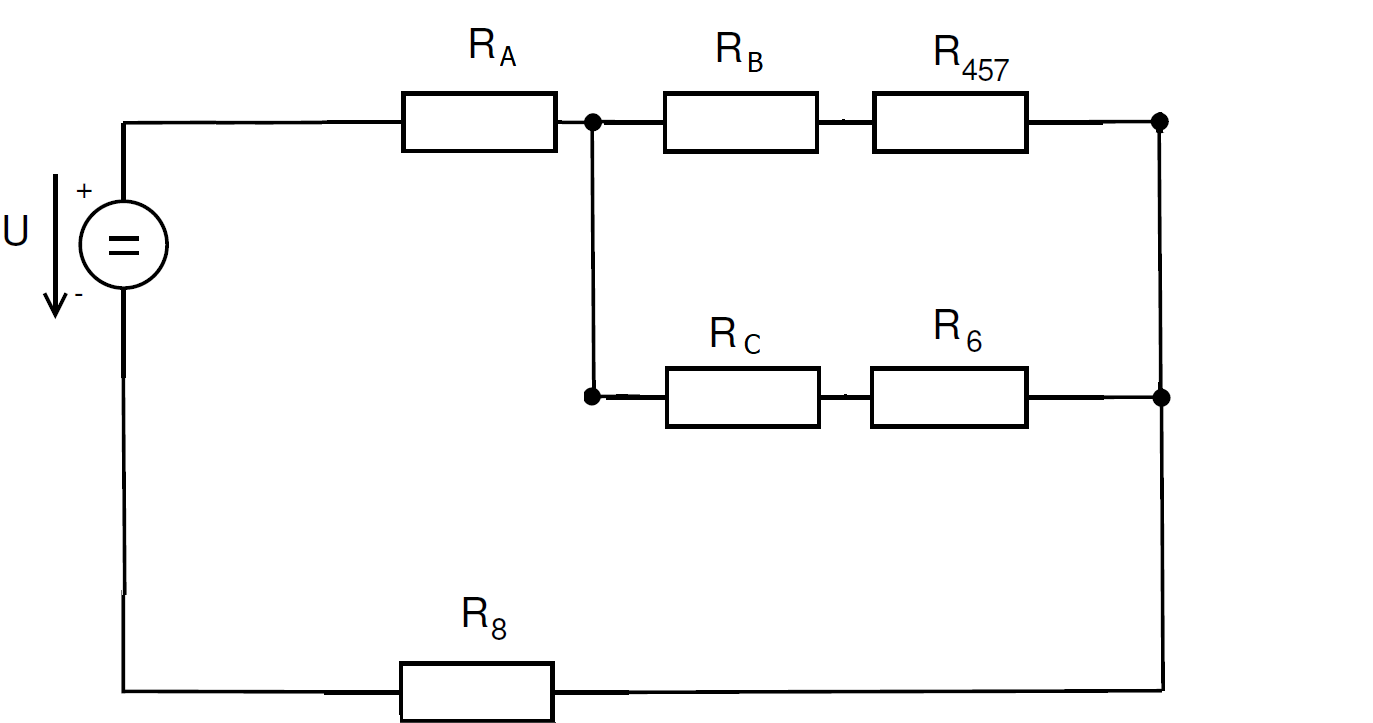
\includegraphics[scale=0.5,keepaspectratio]{fig/obr/Pr1_4.png} \\
\textbf{Krok 4} - Zjednodušenie  $R_{1}$, $R_{2}$ a  $R_{3}$ pomocou rozloženia trojuholníka na hviezdu.
\end{center}

\begin{gather*}
R_{A}=\frac{R_{1} \times R_{2}}{R_{1}+R{2}+R{3}}\\
R_{B}=\frac{R_{1} \times R_{3}}{R_{1}+R{2}+R{3}}\\
R_{C}=\frac{R_{2} \times R_{3}}{R_{1}+R{2}+R{3}}\\
\end{gather*}


%%% Krok 5
\begin{center}
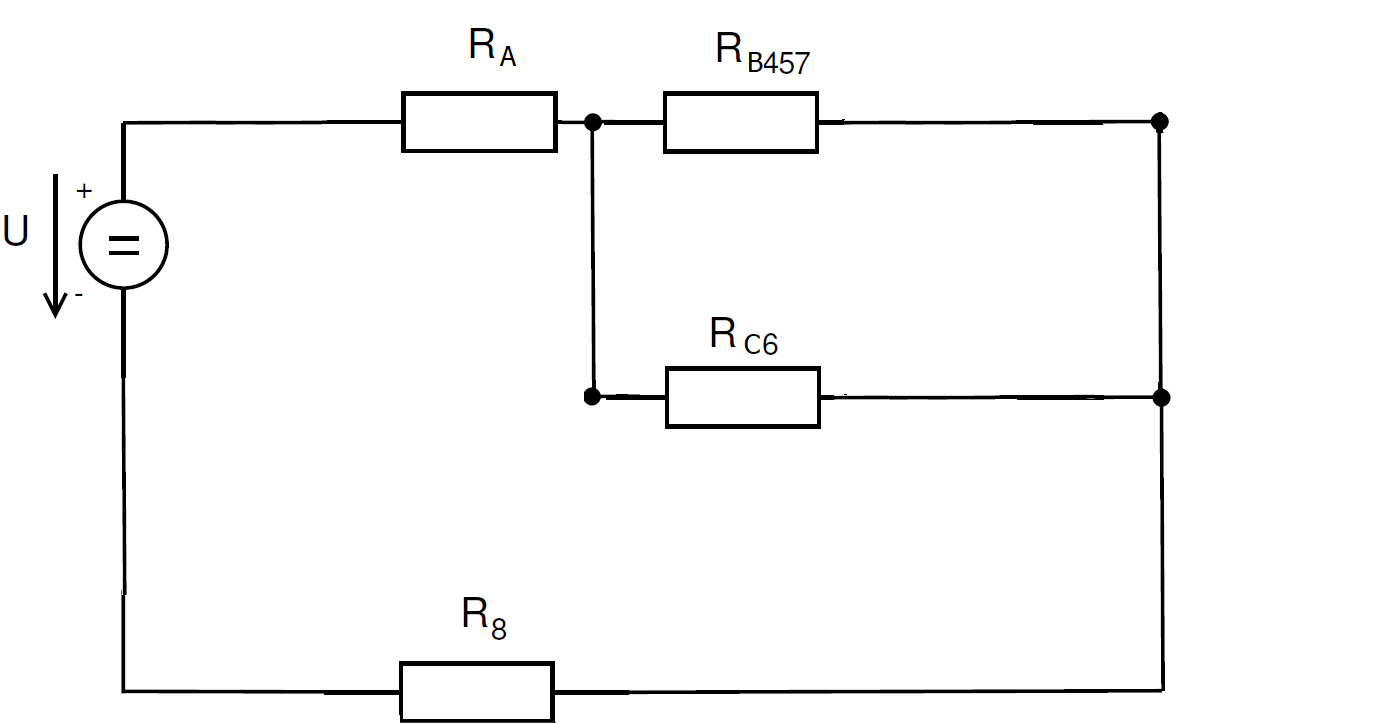
\includegraphics[scale=0.5,keepaspectratio]{fig/obr/Pr1_5.png} \\
\textbf{Krok 5} - Zjednodušenie $R_{B}$ a $R_{457}$ podľa vzorca pre sériovo zapojené rezistory a taktiež zjednodušenie $R_{C}$ a $R_{6}$ podľa vzorca pre sériovo zapojené rezistory.
\end{center}
\newpage
\begin{gather*}
R_{B457}=R_{B}+R_{457}=\frac{R_{1} \times R_{2}}{R_{1}+R_{2}+R_{3}}+R_{457}=\frac{380  \times 330}{380+420+330}+632,47=110,9735+632,4719=743,4454\Omega \\
R_{C6}=R_{C}+R_{6}=\frac{R_{2} \times R_{3}}{R_{1}+R_{2}+R_{3}}+R_{6}=\frac{420 \times 330}{380+420+330}+650=122,6549+650=772,6549\Omega 
\end{gather*}

 
%%% Krok 6 
\begin{center}
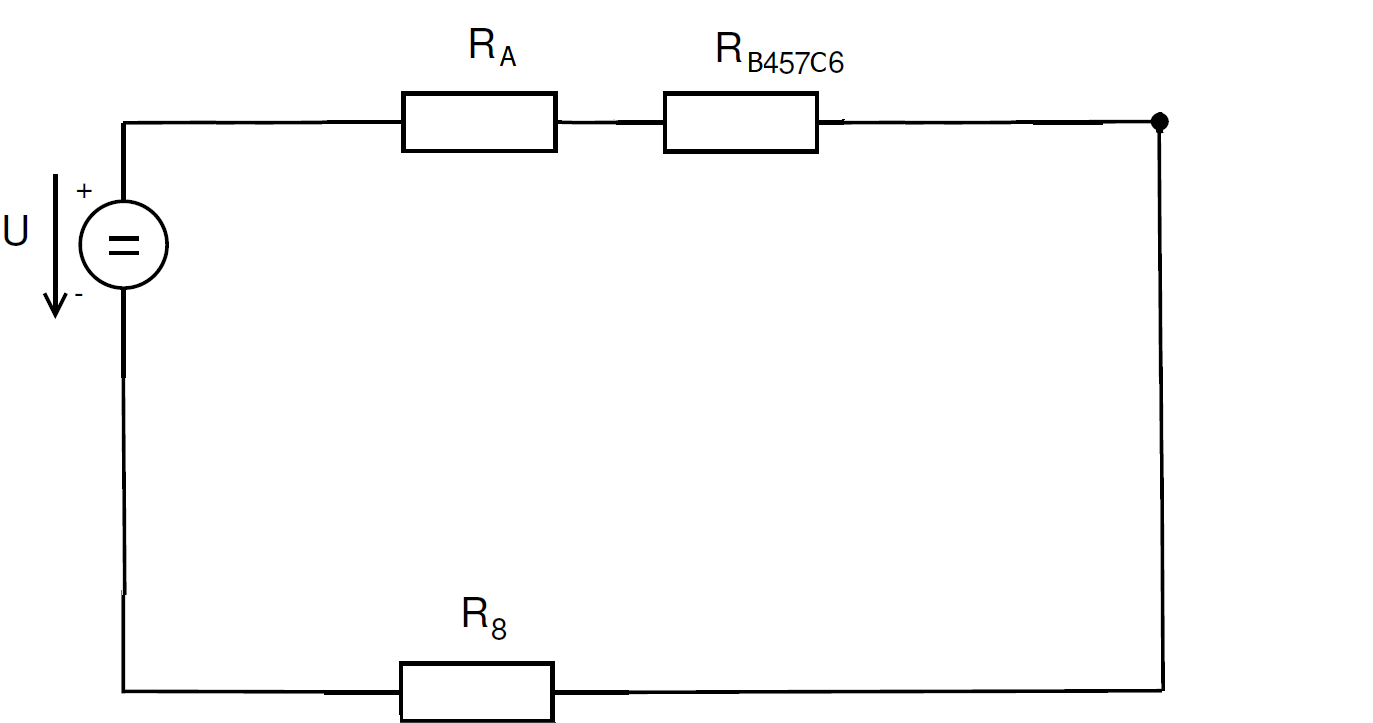
\includegraphics[scale=0.5,keepaspectratio]{fig/obr/Pr1_6.png} \\
\textbf{Krok 6} - Zjednodušenie $R_{B457}$ a $R_{C6}$ podľa vzorca pre paralelne zapojené rezistory.
\end{center}

\begin{gather*}
R_{B457C6}=\frac{R_{B457}  \times R_{C6}}{R_{B457}+R_{C6}}=\frac{743,4454  \times 772,6549}{743,4454+772,6549}=378,8844\Omega 
\end{gather*}


%%% Krok 7
\begin{center}
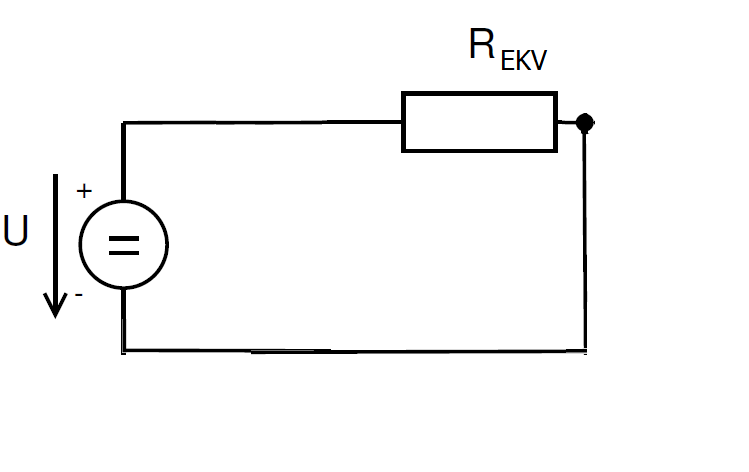
\includegraphics[scale=0.5,keepaspectratio]{fig/obr/Pr1_7.png} \\
\textbf{Krok 7} - Zjednodušenie $R_{A}$, $R_{B457C6}$ a $R_{8}$ podľa vzorca pre sériovo zapojené rezistory.
\end{center}

\begin{gather*}
R_{EKV}=R_{A}+R_{B457C6}+R_{8}=\frac{380 \times 420}{380+420+330}+378,8844+275=795,1233\Omega 
\end{gather*}



%%% Výpočet prúdu
Výpočet prúdu
\begin{gather*}
    % I
    I = \frac{U}{R_{EKV}} = \frac{190}{795,1233} = 0,2390mA \\
\end{gather*}

\newpage

\noindent Teraz spätne dopočítame $\boldsymbol{U_{R5}}$ a $\boldsymbol{I_{R5}}$:
\\\\
Vypočítame si úbytok napätia na $R_{B457C6}$ pomocou prúdu, ktorý sa v sériovom obvode nemení.

\begin{gather*}
    U_{R_{B457C6}} = I \times R_{B457C6} = 0,2390 \times 378,8844 = 90,5534V \\\\
   U_{R_{B457C6}} = U_{R_{B457}}=U_{R_{C6}} \\
\end{gather*}

\noindent Dopočítame si $\boldsymbol I_{R7}$:

\begin{gather*}
    \boldsymbol{I_{R7}} = I_{R_{B457}} = \frac{U_{R_{B457}}}{R_{B457}} =
    \frac{90,5534}{743,4454} =
    \textbf{0,1218A} \\\\
\end{gather*}

\noindent Dopočítame úbytok napätia na $\boldsymbol{U_{R7}}$:

\begin{gather*}
    \boldsymbol{U_{R7}} = I_{R7} \times R_7 = 0,1218 \times 410 = \textbf{49,9380V}
\end{gather*}






